\documentclass[openright]{nitocs}
% \documentclass[openright,draft]{nitocs} % draftを入れると画像が表示されない.下書き時のコンパイル短縮用

%\documentclass[interim]{nitocs}

% \usepackage[dvipdfmx]{graphicx}
\usepackage[dvipdfmx]{graphicx}
\usepackage{latexsym}

\usepackage{bm}

% 数式番号記述
\usepackage{amsmath}
\numberwithin{equation}{section}
\graphicspath{{./IMG/}} % 画像指定用のパス

\renewcommand{\theequation}{\arabic{section}.\arabic{subsection}.\arabic{equation}}
\renewcommand{\thefigure}{\arabic{section}.\arabic{subsection}.\arabic{figure}}
\renewcommand{\thetable}{\arabic{section}.\arabic{subsection}.\arabic{table}}
\makeatletter
\@addtoreset{equation}{section}
\@addtoreset{figure}{section}
\@addtoreset{table}{section}
% 
\def\Underline{\setbox0\hbox\bgroup\let\\\endUnderline}
\def\endUnderline{\vphantom{y}\egroup\smash{\underline{\box0}}\\}
\def\|{\verb|}

\setcounter{page}{1}
\begin{document}

    \title{囲碁における盤面識別システムの検討}  % タイトル
    \etitle{A Study of System for Extracting Go Stone Positions}  % 英語タイトル
    \author{橋本 燎}{Ryo Hashimoto} % 氏名
    \advisor{井上 優良}{Yusuke Inoue}   % 指導教員氏名
    \date{令和3年1月dd日}   % 日付

    \begin{abstract} % 概要
        本研究では,コンピュータと現実での囲碁の対局場面との関係をより親密なものにするために,囲碁盤の画像から碁石の配置を識別するシステムを検討する.システムは,指定した四隅の座標をもとに碁盤を切り抜き,グレースケール変換を行った後に,石を設置できる座標の色情報から石の検出を行う.\\
    \end{abstract}

    \begin{keyword} % キーワード
        画像処理,射影変換,変更確認用に追記
    \end{keyword}


    \maketitle

    % セクション.序論
    % https://www.google.com/url?sa=t&rct=j&q=&esrc=s&source=web&cd=&ved=2ahUKEwj58aT9i4ruAhXTZt4KHcLBBQIQFjAGegQICRAC&url=https%3A%2F%2Fipsj.ixsq.nii.ac.jp%2Fej%2F%3Faction%3Drepository_action_common_download%26item_id%3D90404%26item_no%3D1%26attribute_id%3D1%26file_no%3D1&usg=AOvVaw2sTiUa2iijA6FG63LerTuI
    \section{緒言}  
    \label{sec:format}
            % 前書き
            % 囲碁・棋譜について(もうちょっと説明が欲しい,けど書くことが無い)
        囲碁は,2人のプレイヤーが,「碁石」と呼ばれる白黒の石を,通常$19\times19$の格子が描かれた「碁盤」と呼ばれる板へ交互に配置するボードゲームである.
        他のボードゲームと比較すると,ルール上の制約が極めて少ないといった特徴を持ち,他のボードゲームよりも可能な局面の数は膨大になる(約$2.081681994 \times 10^{170}$通り\cite{numbers}).

            % ここもっと書きたい.コンピュータと囲碁の関係とか.最近AIとかで盛んになってきてることとか.(ただ良さげな参考文献が無い!!)
            % 『コンピュータ囲碁研究』(https://www.jstage.jst.go.jp/article/jjsai/10/6/10_860/_pdf/-char/ja)
        コンピュータの世界においては,囲碁の研究は1960年代から行われていた.
        最も古い研究は,1962年のRemusによる研究``{\it Simulation of a Learning Machine for Playing GO}''\cite{Remus}とされている.
        1969年には,Zobristが世界で初めて囲碁が動作するコンピュータプログラムを作った\cite{Zobrist}.
        2005年には,モンテカルロ木探索を実装した囲碁プログラム``{\it Crazy Stone}''\cite{CrazyStone}が様々な大会で優秀な成績を記録し,以降のコンピュータ囲碁プログラムでも同様のアルゴリズムを採用するなど,コンピュータ囲碁の研究開発に大きな進歩をもたらした.
        2008年には,モンテカルロ木探索を採用した囲碁プログラム``{\it MoGo}''が初めて,公の場でプロ棋士に対して9路盤($9\times9$の囲碁盤で行われる対局)で勝利を収めた\cite{mogo}.
        2015年には,Google DeepMind社が開発した,ニューラルネットワークを実装した以後プログラム``{\it AlphaGo}''が,初めてプロ棋士に対しハンデ無しの対局で勝利した.コンピュータが人間に打ち勝つのは難しいとされていた分野で勝利を果たしたことは,人工知能の有用性を広く知らしめるものとなった.

        % 上での話からここへのつなげ方が思いつかない.こんなにいきなり「本研究では……」なんて入り方はどうなんだろう
        % 本研究について (目的……コンピュータと囲碁の関係をより親密なものにするために? 棋譜の記録の作成を自動化するために? どうしよう)
            %TODO ここ,だいぶ唐突に話が変わったので,説明を増やそう.
            %?     ・なぜ親密にしようと考えたのか
            %?     ・コンピュータと現実の対局を親密にする,っていうのはどういうのをイメージしているのか.
            %? があると分かりやすくなるかな
        本研究では,コンピュータと現実での囲碁の対局をより親密なものにするために,対局中の囲碁の画像から碁石の配置を識別するシステムの検討を行う.
            % 段落変更対策
        具体的には,盤面を含む画像から射影変換を用いて盤面を切り抜き,ノイズ処理を適用して盤面上の線を曖昧なものにした後に,輝度値をもとに碁石の配置を識別するシステムの構築を行う.
        その後,複数の画像に対してシステムを試し,結果を考察する.

            % 論文構成について
        本論文の構成は次の通りである.
        第2章では先行研究についての説明を行う.
        第3章では実験で用いる射影変換とメディアンフィルタ,しきい値の評価で用いた感度と特異度についての説明を行う.
        第4章ではシステムが行う処理についての説明,具体的には射影変換を利用した画像の変形,メディアンフィルタを用いたノイズ除去,石を置くことができる座標の色情報をもとにした碁石の検出を行う.
        第5章では複数の画像に対してシステムを適用し,結果を考察する.
        最後に第6章で本論文をまとめ,今後の課題について述べる.

    \section{先行研究} % セクション.先行研究
        棋譜の自動生成に関する既存研究に着目すると,1手前の着手と比較することで碁石の配置を検出する研究がある.
        芝らは,着手ごとのグレイ画像と1手前のグレイ画像との,碁盤領域内の差分をとることで,碁盤上の碁石の位置(碁石座標)を検出する手法を提案した\cite{PilotStudy}.
        
            %TODO「なんでこの方法でやろうと思ったのか書けるといいね.」
        本研究では,直前の着手の情報を使用せず,1つの着手の画像だけで碁石の位置を検出することを目的とする.

    \section{理論} % セクション.理論
    \label{config}
        \subsection{変換}
            \subsubsection{同次座標}
                座標$(x,y)$に対し,その要素を1つ増やした座標$(\xi_1,\xi_2,\xi_3)$を,以下の関係式を満たすように定義する.\\
                \begin{equation} % 同次座標の数式
                    \begin{split} % 複数行に1つの式番号を与える
                        x = \frac{\xi_1}{\xi_3} \\ 
                        y = \frac{\xi_2}{\xi_3}
                    \end{split}
                    \label{Homogeneous}
                \end{equation}

                ただし,$\xi_1,\xi_2,\xi_3$のうち,少なくとも1つは0ではないとする.このように定義される座標を同次座標と呼ぶ\cite{Homogenous}.

                同次座標においては,$\lambda\neq0$なる任意の$\lambda$に対して,$(\xi_1,\xi_2,\xi_3)$と$(\lambda\xi_1,\lambda\xi_2,\lambda\xi_3)$は,通常の座標に直したとき,ともに$(\xi_1/\xi_3,\xi_2/\xi_3)$となるため,同じ点を表している.つまり,同次座標による表現では,定数倍をしても変わらないとみなすことができる.このような表現を同値であるとよび,これを式では以下のように表す.
                \begin{equation} % 同次座標の数式2
                    \left(
                        \begin{array}{ccc}
                            \xi_1\\
                            \xi_2\\
                            \xi_3
                        \end{array}
                    \right) \sim % \sim: 「~」
                    \left(
                        \begin{array}{ccc}
                            \lambda\xi_1\\
                            \lambda\xi_2\\
                            \lambda\xi_3
                        \end{array}
                    \right)
                \end{equation}
                ここで,記号$\sim$が同値関係を表し,定数倍の違いを許して等しいことを意味する.

            \subsubsection{射影変換}
                同次座標を利用することにより,一般的な変換を表現することができる.これは以下の式で表現されるもので,射影変換と呼ばれている.
                \begin{equation} % 射影変換の数式
                    \left(
                        \begin{array}{ccc}
                        x'\\
                        y'\\
                        1
                        \end{array}
                    \right)\sim
                    \left(
                        \begin{array}{ccc}
                        h_{11} & h_{12} & h_{13}\\
                        h_{21} & h_{22} & h_{23}\\
                        h_{31} & h_{32} & h_{33}\\
                        \end{array}
                    \right)
                    \left(
                        \begin{array}{ccc}
                        x\\
                        y\\
                        1
                        \end{array}
                    \right)
                    \label{Homography}
                \end{equation}
                あるいは,これをベクトルと行列の記号を用いて,以下のように表現することもできる.
                \begin{equation}
                    \bm{\vec{x}'} \sim \bm{H\vec{x}}
                \end{equation}
                $\bm{H}$は任意の$3\times3$の行列である.

                式(\ref{Homogeneous})の関係を用いて,(\ref{Homography})から座標$(x',y')$を求めると以下のようになる.
                \begin{equation} % 変換行列を用いてx,yを表現する式
                    \begin{split} % 複数行に1つの式番号を与える
                        x' = \frac{h_{11}x+h_{12}y+h_{13}}{h_{31}x+h_{32}y+h_{33}} \\ 
                        y' = \frac{h_{21}x+h_{22}y+h_{23}}{h_{31}x+h_{32}y+h_{33}} \\ 
                    \end{split}
                \end{equation}

                射影変換においては,線分の直線性は保たれるものの,平行性は失われる.別の言い方をすると,任意の四角形を別の任意の四角形に移すような変換であるといえる.

        % 2.2
        \subsection{メディアンフィルタ}
            領域内の画素値の中央値(メディアン)を出力とするフィルタをメディアンフィルタと呼ぶ.
            このフィルタは,コントラストの差がある輪郭部分がぼやけにくい特徴を持つ.
            特定の画像に対して,領域内の画素値の平均を出力するフィルタ(平均化フィルタ)とメディアンフィルタを施した一例を,それぞれ図\ref{sample_average},図\ref{sample_median}に示す.
            \begin{figure}[htbp] % 平均化フィルタ,メディアンフィルタの2枚
                \begin{center}
                  \begin{tabular}{c}
                    \begin{minipage}{0.5\hsize}
                      \begin{center}
                        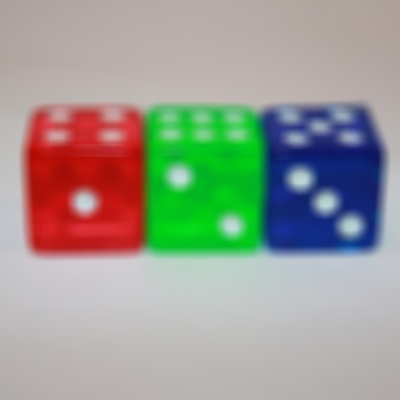
\includegraphics[width=32mm,height=32mm]{sample_average.jpg}
                    \caption{平均化フィルタ}
                    \label{sample_average}
                      \end{center}
                    \end{minipage}
                    \begin{minipage}{0.5\hsize}
                      \begin{center}
                        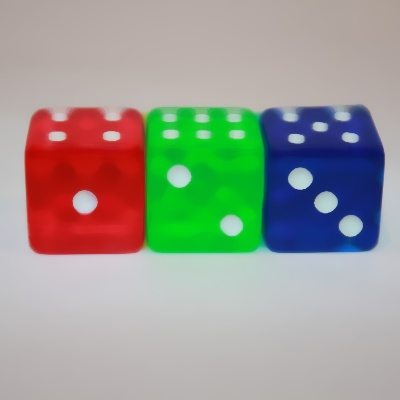
\includegraphics[width=32mm,height=32mm]{sample_median.jpg}
                    \caption{メディアンフィルタ}
                    \label{sample_median}
                      \end{center}
                    \end{minipage}
                  \end{tabular}
                \end{center}
            \end{figure}

        \subsection{感度} % 真陽性率
            % https://jeaweb.jp/files/about_epi_research/contest2016_1_202007.pdf
            % https://bellcurve.jp/statistics/glossary/2014.html (こっちのほうが分かりやすいけど,参考文献には不適切な気がする.)
        検査で検出したい信号や疾患を有するもののうち,検査が正しく陽性と判断したものの割合を指す.
        真陽性率(TPF: True Positive Fraction)とも呼ぶ.

        \subsection{特異度} % 真陰性率
        検査で検出したい信号や疾患を有さないもののうち,検査が正しく陰性と判断したものの割合を指す.
        真陰性率(TNF: True Negative Fraction)とも呼ぶ.

    \section{盤面識別システム} % セクション.システムについて
            %TODO この章はもっと書けると思うので,全体的に説明を拡充しましょう!
                %! 目標は,後で他の人が同じ実験をできるように説明する,です
        本研究で検討したシステムでは,盤面を含む画像から,碁石の位置を識別することを目的とする.

        実際には,盤面を含む画像から盤面を切り抜き,碁石上の線を黒石と誤検知しないようノイズ処理を施した後に$19\times19$の領域を付与する.その後,付与した領域内における輝度値の平均を計算し,黒石・白石のしきい値とを比較,結果をもとに石の識別を行う.
        システムの流れを図\ref{flow}に示す.
            % 図番号が4.0.1になってる.0はマズい?
            %! 図の番号付け,執筆の最後でいいので整えてください.4.0.1 -> 4.1.2 って変なので.
        \begin{figure} % フロー図
            \begin{center}
            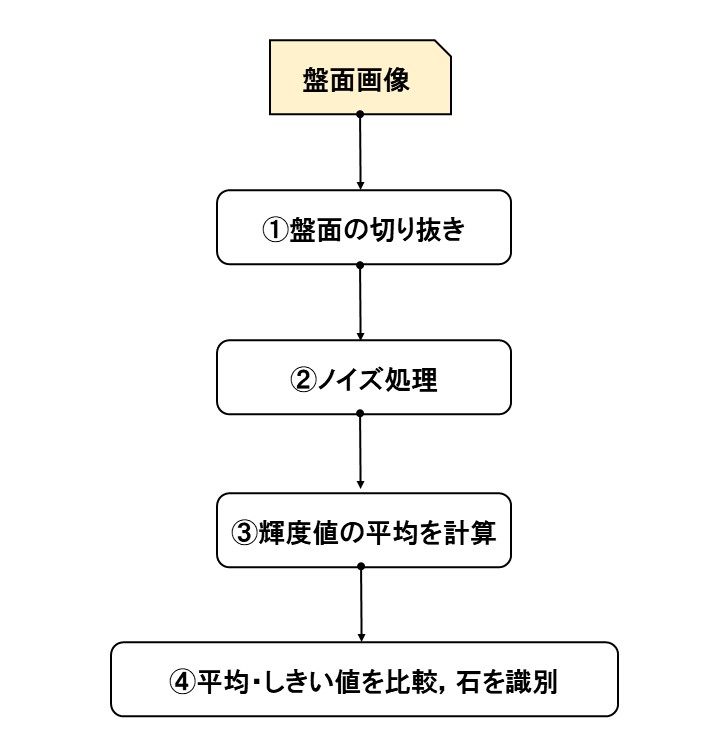
\includegraphics[width=72mm,height=75.6mm]{flow.jpg} 
            \caption{フロー図}
            \label{flow}
            \end{center}
        \end{figure}

        \subsection{切り抜き}
            盤面画像の生成には,碁盤の頂点座標と,変換後の四角形の頂点座標を指定して変換行列を生成し,その行列を用いて射影変換を行う.変換前と変換後の図を図\ref{cornerImg},図\ref{boardImg}に示す.
            \begin{figure} % 射影変換前の画像
                \begin{center}
                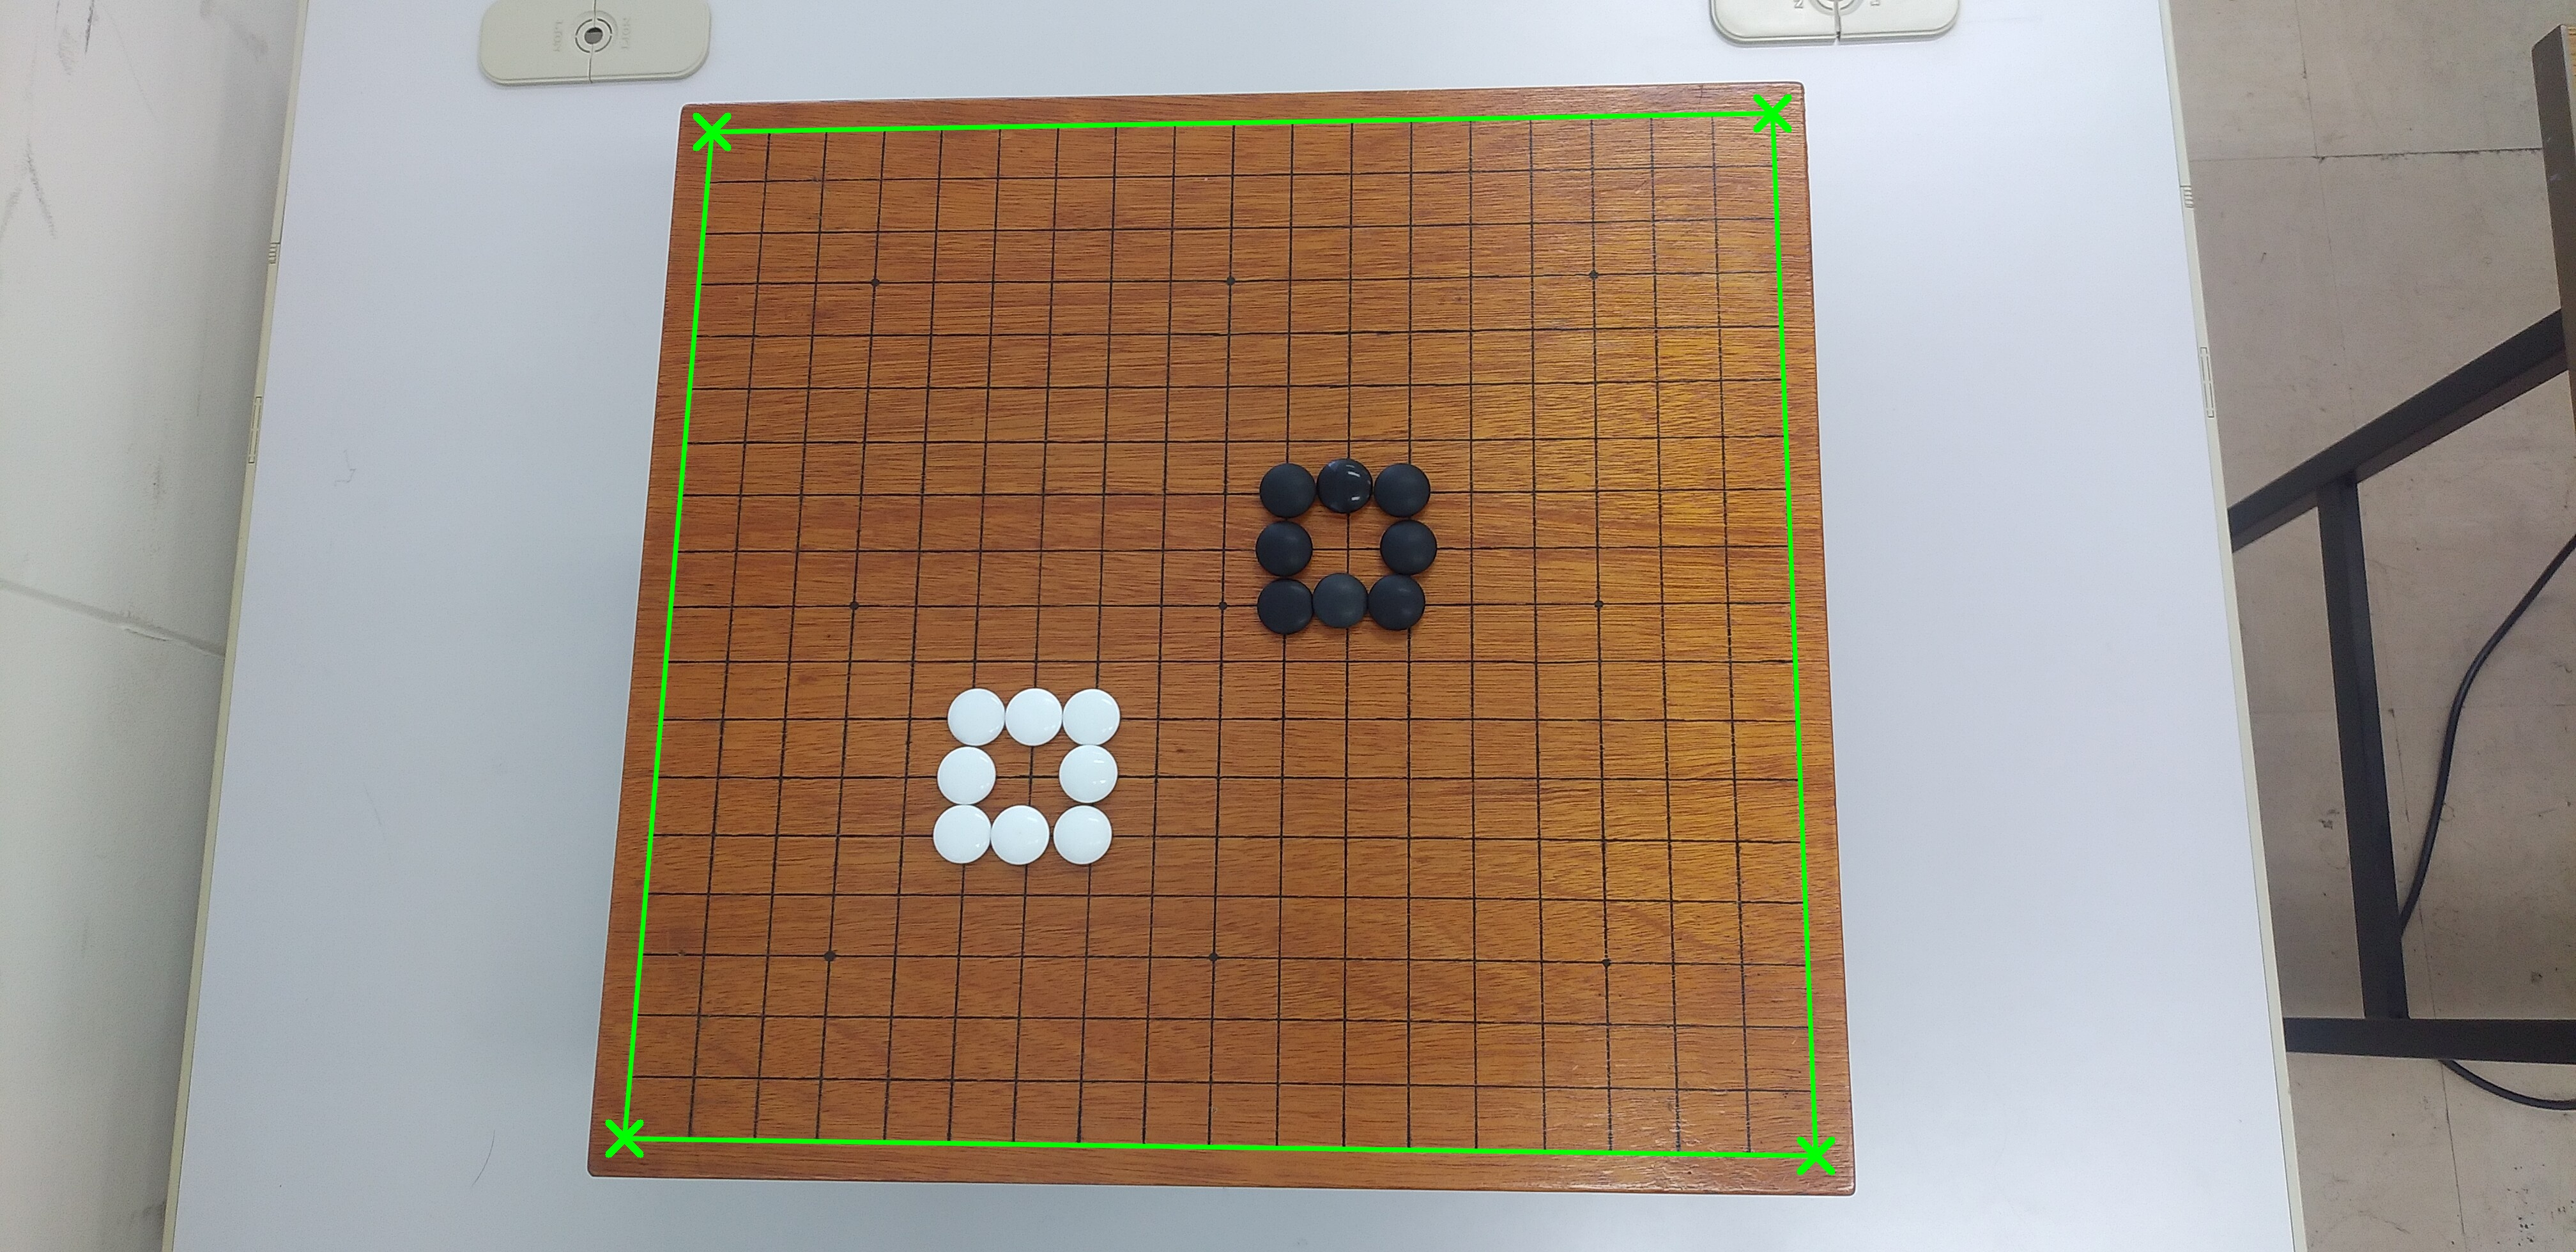
\includegraphics[width=72mm,height=35mm]{cornerImg.jpg} 
                \caption{射影変換前}
                \label{cornerImg}
                \end{center}
            \end{figure}
            \begin{figure} % 射影変換後の画像
                \begin{center}
                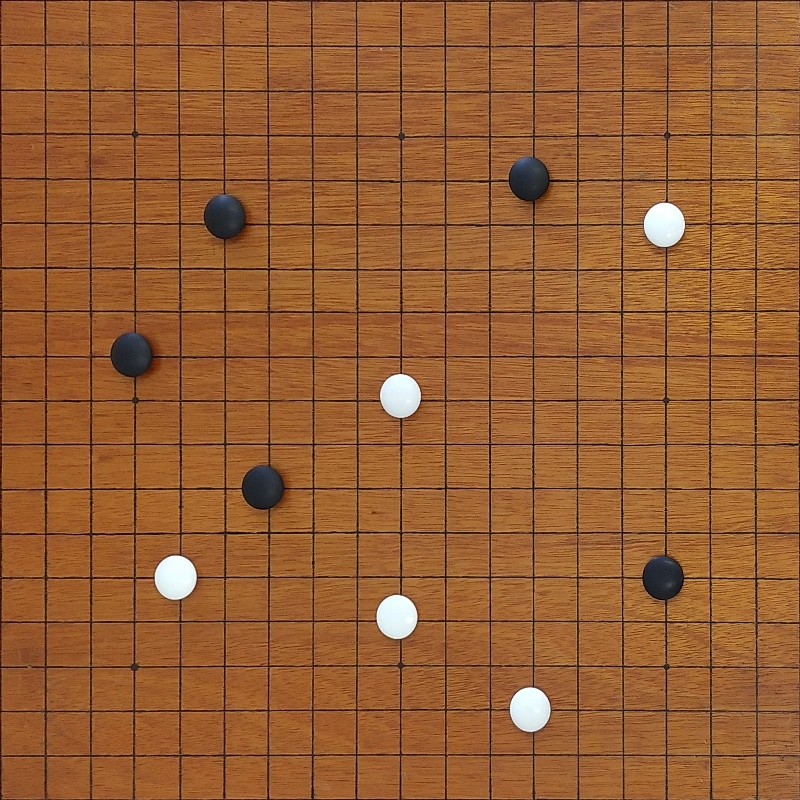
\includegraphics[width=50mm,height=50mm]{boardImg.jpg} 
                \caption{射影変換後}
                \label{boardImg}
                \end{center}
            \end{figure}

        \subsection{ノイズ除去}
            4.1で生成した画像(図\ref{boardImg})に対し,碁盤上の線を消すために,メディアンフィルタを用いてノイズ処理を行う.処理結果を図\ref{noiseReduced}に示す.
            \begin{figure} % ノイズ除去後の盤面
                \begin{center}
                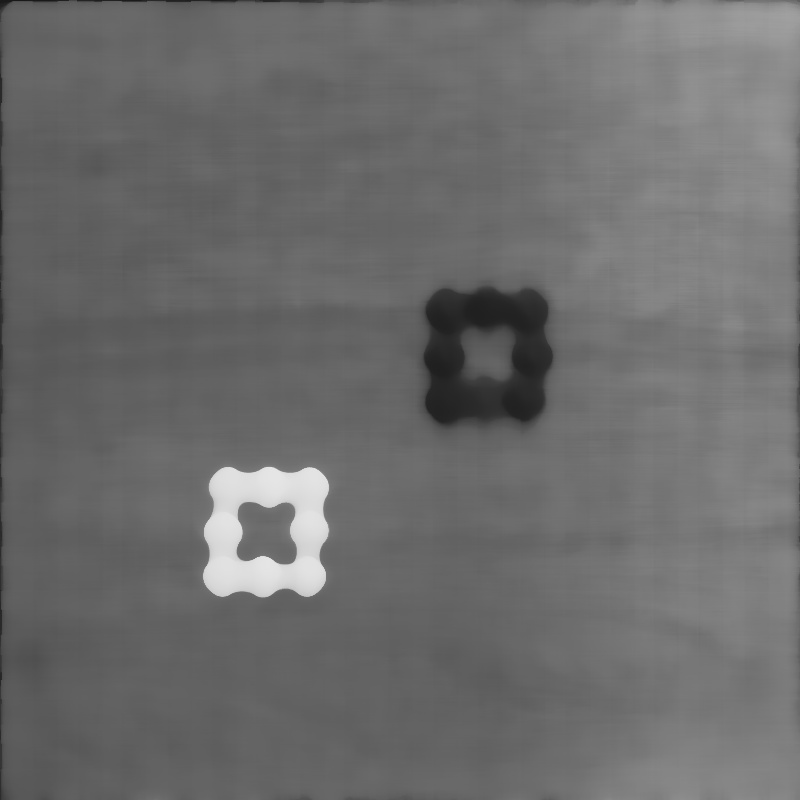
\includegraphics[width=50mm,height=50mm]{noiseReducedImg.jpg} 
                \caption{ノイズ除去後の盤面}
                \label{noiseReduced}
                \end{center}
            \end{figure}

        \subsection{領域の付与}
            \label{area}
            4.2(図\ref{noiseReduced})に対し,等間隔に$19\times19$個の小さな領域を付与する.領域を可視化した図を図\ref{boardWithArea}に示す.
            \begin{figure} % 領域を可視化した図
                \begin{center}
                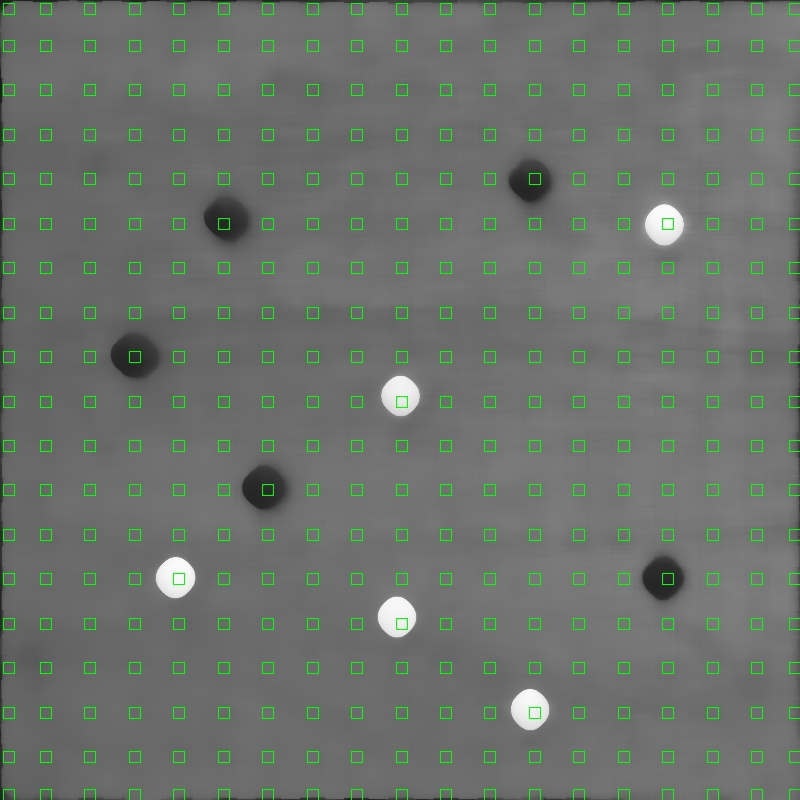
\includegraphics[width=50mm,height=50mm]{boardWithAreaImg.jpg} 
                \caption{領域を可視化した盤面}
                \label{boardWithArea}
                \end{center}
            \end{figure}

        \subsection{識別} \label{identify}  
            \ref{area}で与えた領域内の輝度値の平均(0~255)を取得し,設定したしきい値をもとに,各領域を
            \begin{itemize} % 3種類
                \item 平均値が黒石のしきい値より小さい = 「黒石がある」
                \item 平均値が白石のしきい値より大きい = 「白石がある」
                \item それ以外
            \end{itemize}
            の3種類に分類する.
            %! この下の図は必要か? PDFじゃなく印刷提出なら白黒印刷するはずだし,いらない気もする.
            実際に識別した結果を図\ref{result}に示す.

            \begin{figure} % 領域を可視化した図
                \begin{center}
                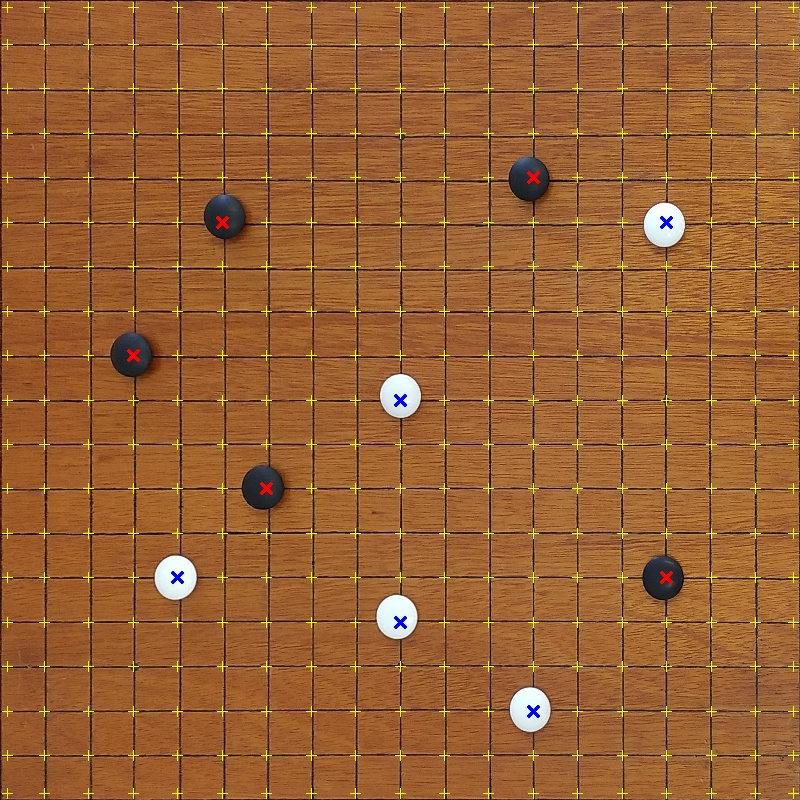
\includegraphics[width=50mm,height=50mm]{result.jpg} 
                \caption{識別結果を重ねた盤面}
                \label{result}
                \end{center}
            \end{figure}


    \section{実験と考察} % セクション.実験
            %TODO 実験の目的をこの章のどこかに書こう
                %? 研究の目的(碁石の位置認識)を実現するために,何を明らかにしようと思ってこの実験をやったんだっけ,というのを書いてほしいな.
                %? (逆に言うと,何を明らかにすれば碁石の位置認識を実現できた!と言える?)
        この章では,システムの有効性を検証するため,実際に盤面を含む画像を使ってシステムを適用し,結果を考察する.

        \subsection{しきい値の決定} \label{threshold}
            今回の実験で用いるしきい値は,2枚の盤面画像(図\ref{DSC0087},図\ref{DSC0100})に対し,さまざまなしきい値に応じた感度と特異度をもとに,最適なしきい値を決定した.
            図\ref{DSC0087},図\ref{DSC0100}における黒石の感度と特異度をそれぞれ図\ref{Case1Black}と図\ref{Case2Black}に,
            白石の感度と特異度をそれぞれ図\ref{Case1White}と図\ref{Case2White}に示す.

            図\ref{Case1Black}と図\ref{Case2Black}より,図\ref{DSC0087}と図\ref{DSC0100}の両方に対して,黒石のしきい値は52で感度100\%,特異度100\%を記録したため,今回の実験では52を使用した.

            図\ref{Case1White},図\ref{Case2White}より,図\ref{DSC0087}と図\ref{DSC0100}の両方に対して,白石のしきい値は156~160の範囲で感度100\%,特異度100\%を記録したため,今回の実験ではその範囲の中央値である158を使用した.
            \begin{figure} % DSC_0087
                \begin{center}
                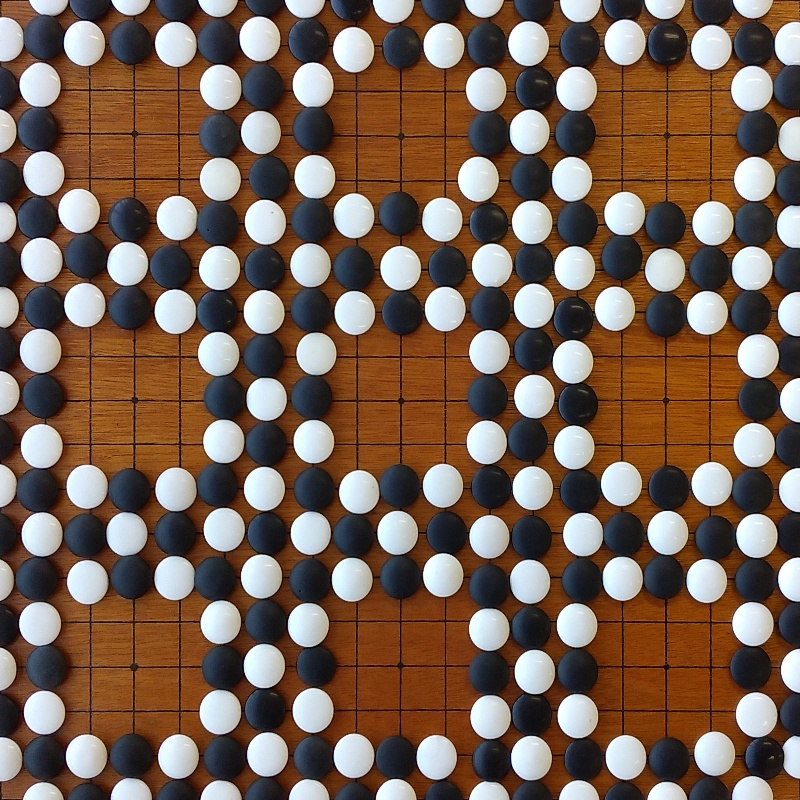
\includegraphics[width=50mm,height=50mm]{DSC_0087/boardImg.jpg} 
                \caption{しきい値の決定に用いた盤面1}
                \label{DSC0087}
                \end{center}
            \end{figure}

            \begin{figure} % DSC_0100
                \begin{center}
                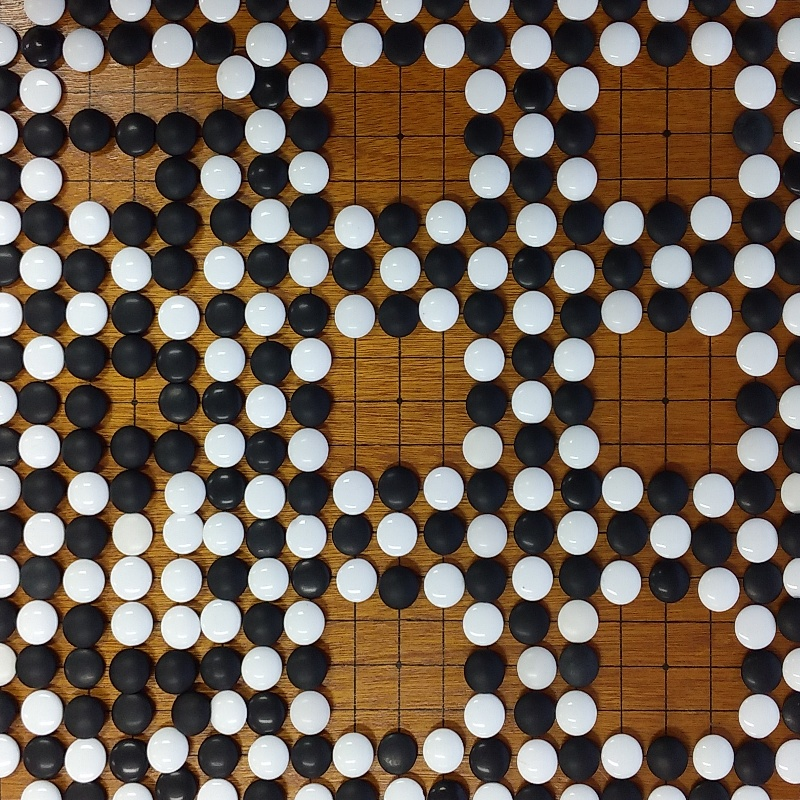
\includegraphics[width=50mm,height=50mm]{DSC_0100/boardImg.jpg} 
                \caption{しきい値の決定に用いた盤面2}
                \label{DSC0100}
                \end{center}
            \end{figure}

            \begin{figure} % 黒石の感度・特異度1
                \begin{center}
                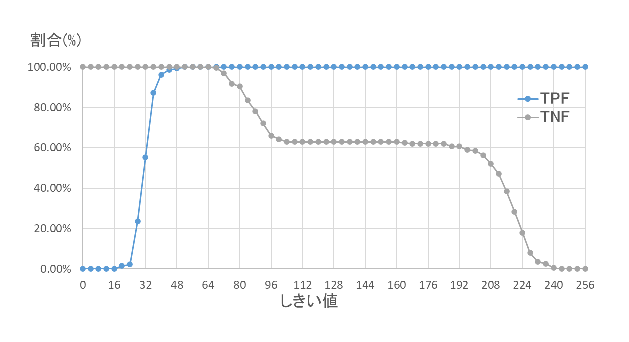
\includegraphics[width=80mm,height=40mm]{Case1_Black_TPF_TNF.eps} 
                \caption{黒石の感度・特異度1}
                \label{Case1Black}
                \end{center}
            \end{figure}

            \begin{figure} % 黒石の感度・特異度2
                \begin{center}
                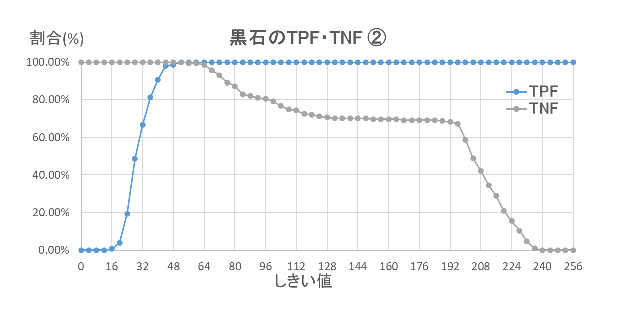
\includegraphics[width=80mm,height=40mm]{Case2_Black_TPF_TNF.eps} 
                \caption{黒石の感度・特異度2}
                \label{Case2Black}
                \end{center}
            \end{figure}

            \begin{figure} % 白石の感度・特異度1
                \begin{center}
                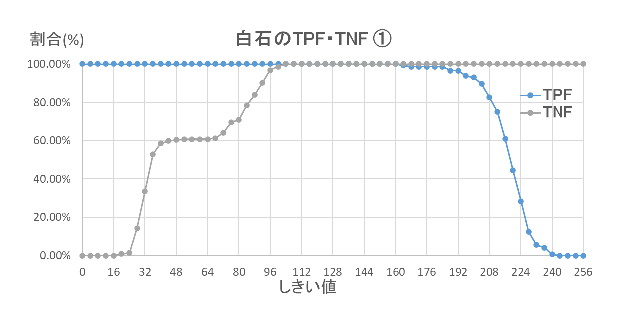
\includegraphics[width=80mm,height=40mm]{Case1_White_TPF_TNF.eps} 
                \caption{白石の感度・特異度1}
                \label{Case1White}
                \end{center}
            \end{figure}
            
            \begin{figure} % 白石の感度・特異度2
                \begin{center}
                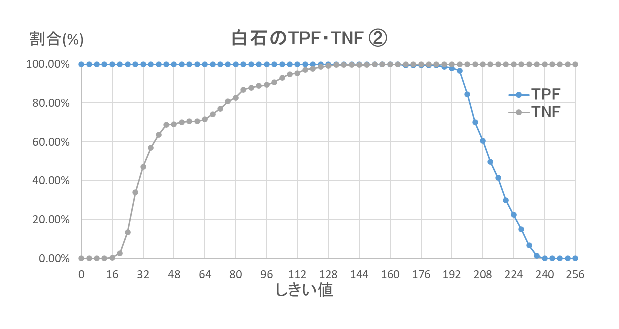
\includegraphics[width=80mm,height=40mm]{Case2_White_TPF_TNF.eps} 
                \caption{白石の感度・特異度2}
                \label{Case2White}
                \end{center}
            \end{figure}

        \subsection{事例1}
            正しく取得できた場合について説明

            画像を多用してページ数を稼ぎたいところだけど,ただでさえ画像が多いからこれ以上増やすと見栄えが悲惨なことになりそう……

        \subsection{事例2}
            異常が多発する(反射・配置ズレが多い)場合について説明

    \section{結言}\label{sec:Item} % 結言
        本文

        まとめと,今後の課題とか?

            
            

    \begin{thebibliography}{10} % 参考文献

        % Webサイトの参考文献の書き方が怪しい.確認を取ること!

            % 書き方に困ったやつ.そもそもこの情報あってもなくてもいいやつ?
            % https://tromp.github.io/go/legal.html
        \bibitem{numbers}
        Number of legal Go positions

            % 他の論文での参考文献をそのままコピーした.
        \bibitem{Remus}
        Remus, H. : 
        {\it Simulation of a Learning Machine for Playing Go}, 
        Information Processing, 
        pp. 192-194 (1962). 

        \bibitem{Zobrist}
        Zobrist, A. L.: 
        {\it A Model of Visual Organisation for the Game of Go}, 
        Proceedings of AFIPS Spring joint Computer Conference, 
        Vol. 34, pp. 103-112 (1969). 

            % 書き方に困ったやつ
            % https://www.remi-coulom.fr/CrazyStone/
        \bibitem{CrazyStone}
        Rémi Coulom「Crazy Stone」

        \bibitem{mogo}
        美添一樹(2008)「モンテカルロ木探索 ―コンピュータ囲碁に革命を起こした新手法」,『情報処理』,49(6),pp.686-693

            % 書き方に困ったやつ
            % https://deepmind.com/research/case-studies/alphago-the-story-so-far
        \bibitem{AlphaGo}
        DeepMind「AlphaGo」

        \bibitem{PilotStudy}
        芝 浩二郎・古屋 保・西 省吾・森 邦彦(2006)「画像処理による囲碁棋譜自動生成システム」,  『電気学会論文誌C(電子・情報・システム部門誌)』, 126(8), pp.980-989.

        % 小澤菜月先輩の論文「GANを用いた編み図ジェネレータの構成のための検討」の参考文献をパクった
        \bibitem{Homogenous}
        ディジタル画像処理[改訂第二版],松阪 喜幸(2020)

        % \bibitem{total}
        % 伊藤和人: \LaTeX トータルガイド,秀和システムトレーディング (1991).
        % \bibitem{nodera}
        % 野寺隆志:楽々 \LaTeX,共立出版 (1990).

        % \bibitem{okumura}
        % 奥村晴彦:改訂第5版 \LaTeXe 美文書作成入門,
        % 技術評論社(2010).

        % \bibitem{companion}
        % Goossens, M., Mittelbach, F. and Samarin, A.:
        % {\it The LaTeX Companion},
        % Addison Wesley, Reading, Massachusetts (1993).

        % \bibitem{book1}
        % 木下是雄:
        % 理科系の作文技術,
        % 中公新書(1981).

        % \bibitem{book2}
        % Strunk W. J. and White E.B.:
        % {\it The Elements of Style, Forth Edition},
        % Longman (2000).

        % \bibitem{book3}
        % Blake G. and Bly R.W.:
        % {\it The Elements of Technical Writing},
        % Longman (1993).

        % \bibitem{book4}
        % Higham N.J.:
        % {\it Handbook of Writing for the Mathematical Sciences},
        % SIAM (1998).

    \end{thebibliography}

\end{document}